% Options for packages loaded elsewhere
\PassOptionsToPackage{unicode}{hyperref}
\PassOptionsToPackage{hyphens}{url}
%
\documentclass[
  12 pt,
]{article}
\usepackage{lmodern}
\usepackage{amssymb,amsmath}
\usepackage{ifxetex,ifluatex}
\ifnum 0\ifxetex 1\fi\ifluatex 1\fi=0 % if pdftex
  \usepackage[T1]{fontenc}
  \usepackage[utf8]{inputenc}
  \usepackage{textcomp} % provide euro and other symbols
\else % if luatex or xetex
  \usepackage{unicode-math}
  \defaultfontfeatures{Scale=MatchLowercase}
  \defaultfontfeatures[\rmfamily]{Ligatures=TeX,Scale=1}
\fi
% Use upquote if available, for straight quotes in verbatim environments
\IfFileExists{upquote.sty}{\usepackage{upquote}}{}
\IfFileExists{microtype.sty}{% use microtype if available
  \usepackage[]{microtype}
  \UseMicrotypeSet[protrusion]{basicmath} % disable protrusion for tt fonts
}{}
\makeatletter
\@ifundefined{KOMAClassName}{% if non-KOMA class
  \IfFileExists{parskip.sty}{%
    \usepackage{parskip}
  }{% else
    \setlength{\parindent}{0pt}
    \setlength{\parskip}{6pt plus 2pt minus 1pt}}
}{% if KOMA class
  \KOMAoptions{parskip=half}}
\makeatother
\usepackage{xcolor}
\IfFileExists{xurl.sty}{\usepackage{xurl}}{} % add URL line breaks if available
\IfFileExists{bookmark.sty}{\usepackage{bookmark}}{\usepackage{hyperref}}
\hypersetup{
  pdftitle={Amazon Network Analysis},
  pdfauthor={Ferdinand Bubeck},
  hidelinks,
  pdfcreator={LaTeX via pandoc}}
\urlstyle{same} % disable monospaced font for URLs
\usepackage[margin=1in]{geometry}
\usepackage{color}
\usepackage{fancyvrb}
\newcommand{\VerbBar}{|}
\newcommand{\VERB}{\Verb[commandchars=\\\{\}]}
\DefineVerbatimEnvironment{Highlighting}{Verbatim}{commandchars=\\\{\}}
% Add ',fontsize=\small' for more characters per line
\usepackage{framed}
\definecolor{shadecolor}{RGB}{248,248,248}
\newenvironment{Shaded}{\begin{snugshade}}{\end{snugshade}}
\newcommand{\AlertTok}[1]{\textcolor[rgb]{0.94,0.16,0.16}{#1}}
\newcommand{\AnnotationTok}[1]{\textcolor[rgb]{0.56,0.35,0.01}{\textbf{\textit{#1}}}}
\newcommand{\AttributeTok}[1]{\textcolor[rgb]{0.77,0.63,0.00}{#1}}
\newcommand{\BaseNTok}[1]{\textcolor[rgb]{0.00,0.00,0.81}{#1}}
\newcommand{\BuiltInTok}[1]{#1}
\newcommand{\CharTok}[1]{\textcolor[rgb]{0.31,0.60,0.02}{#1}}
\newcommand{\CommentTok}[1]{\textcolor[rgb]{0.56,0.35,0.01}{\textit{#1}}}
\newcommand{\CommentVarTok}[1]{\textcolor[rgb]{0.56,0.35,0.01}{\textbf{\textit{#1}}}}
\newcommand{\ConstantTok}[1]{\textcolor[rgb]{0.00,0.00,0.00}{#1}}
\newcommand{\ControlFlowTok}[1]{\textcolor[rgb]{0.13,0.29,0.53}{\textbf{#1}}}
\newcommand{\DataTypeTok}[1]{\textcolor[rgb]{0.13,0.29,0.53}{#1}}
\newcommand{\DecValTok}[1]{\textcolor[rgb]{0.00,0.00,0.81}{#1}}
\newcommand{\DocumentationTok}[1]{\textcolor[rgb]{0.56,0.35,0.01}{\textbf{\textit{#1}}}}
\newcommand{\ErrorTok}[1]{\textcolor[rgb]{0.64,0.00,0.00}{\textbf{#1}}}
\newcommand{\ExtensionTok}[1]{#1}
\newcommand{\FloatTok}[1]{\textcolor[rgb]{0.00,0.00,0.81}{#1}}
\newcommand{\FunctionTok}[1]{\textcolor[rgb]{0.00,0.00,0.00}{#1}}
\newcommand{\ImportTok}[1]{#1}
\newcommand{\InformationTok}[1]{\textcolor[rgb]{0.56,0.35,0.01}{\textbf{\textit{#1}}}}
\newcommand{\KeywordTok}[1]{\textcolor[rgb]{0.13,0.29,0.53}{\textbf{#1}}}
\newcommand{\NormalTok}[1]{#1}
\newcommand{\OperatorTok}[1]{\textcolor[rgb]{0.81,0.36,0.00}{\textbf{#1}}}
\newcommand{\OtherTok}[1]{\textcolor[rgb]{0.56,0.35,0.01}{#1}}
\newcommand{\PreprocessorTok}[1]{\textcolor[rgb]{0.56,0.35,0.01}{\textit{#1}}}
\newcommand{\RegionMarkerTok}[1]{#1}
\newcommand{\SpecialCharTok}[1]{\textcolor[rgb]{0.00,0.00,0.00}{#1}}
\newcommand{\SpecialStringTok}[1]{\textcolor[rgb]{0.31,0.60,0.02}{#1}}
\newcommand{\StringTok}[1]{\textcolor[rgb]{0.31,0.60,0.02}{#1}}
\newcommand{\VariableTok}[1]{\textcolor[rgb]{0.00,0.00,0.00}{#1}}
\newcommand{\VerbatimStringTok}[1]{\textcolor[rgb]{0.31,0.60,0.02}{#1}}
\newcommand{\WarningTok}[1]{\textcolor[rgb]{0.56,0.35,0.01}{\textbf{\textit{#1}}}}
\usepackage{graphicx,grffile}
\makeatletter
\def\maxwidth{\ifdim\Gin@nat@width>\linewidth\linewidth\else\Gin@nat@width\fi}
\def\maxheight{\ifdim\Gin@nat@height>\textheight\textheight\else\Gin@nat@height\fi}
\makeatother
% Scale images if necessary, so that they will not overflow the page
% margins by default, and it is still possible to overwrite the defaults
% using explicit options in \includegraphics[width, height, ...]{}
\setkeys{Gin}{width=\maxwidth,height=\maxheight,keepaspectratio}
% Set default figure placement to htbp
\makeatletter
\def\fps@figure{htbp}
\makeatother
\setlength{\emergencystretch}{3em} % prevent overfull lines
\providecommand{\tightlist}{%
  \setlength{\itemsep}{0pt}\setlength{\parskip}{0pt}}
\setcounter{secnumdepth}{5}
\usepackage{graphicx} \usepackage{fancyhdr} \pagestyle{fancy} \setlength\headheight{28pt} \fancyhead[L]{
\includegraphics[width=2.5cm]{Data/logo.png}} \fancyfoot[LE,RO]{Ferdinand Bubeck}

\title{Amazon Network Analysis}
\usepackage{etoolbox}
\makeatletter
\providecommand{\subtitle}[1]{% add subtitle to \maketitle
  \apptocmd{\@title}{\par {\large #1 \par}}{}{}
}
\makeatother
\subtitle{Assignment im Rahmen der Vorlesung `Social Network Analyis'}
\author{Ferdinand Bubeck}
\date{2021-11-16}

\begin{document}
\maketitle

\renewcommand*\contentsname{Inhaltsverzeichnis}
{
\setcounter{tocdepth}{3}
\tableofcontents
}
\newpage

\hypertarget{einleitung}{%
\section{Einleitung}\label{einleitung}}

Im Rahmen der Vorlesung ``Social Network Analyses'' von Philipp Mendoza
an der DHBW Stuttgart soll eine Netzwerkanalyse auf Basis eines
gewählten Datensatzes abgegeben werden. Der Autor dieser Arbeit hat sich
für einen Amazon Produktdatensatz entschieden, welcher im Laufe der
Arbeit vorgestellt wird.

\hypertarget{zielsetzung}{%
\subsection{Zielsetzung}\label{zielsetzung}}

Zielsetzung ist es, auf Basis der Daten eine Forschungsfrage zu
überlegen und diese netzwerkanalytisch zu beantworten. Dabei sollen
erlernte Konzepte aus der Vorlesung einfließen und mindestens eine
Netzwerk Visualisierung enthalten sein.

\hypertarget{vorgehensweise}{%
\subsection{Vorgehensweise}\label{vorgehensweise}}

Als Vorgehensweise wird in diesem Projekt das für das Feld Data Science
etablierte Standard-Vorgehen CRISP-DM gewählt (Cross Industry Standard
Process for Data Mining). In mehreren Phasen werden so von dem richtigen
Verständnis der Daten, dem Data Wrangling und Data Preprocessing bis hin
zum Modelfitting und der Evaluation alle entscheidenen Schritte
strukturiert durchlaufen, um ein optimales Ergebnis aus den Daten zu
generieren. In der Abbildung 1 ist das Vorgehensmodell abgebildet. Da es
sich in diesem Projekt um ein PoC handelt, wird die letzte Phase
`Deployment' ausgelassen.

\begin{figure}
\centering
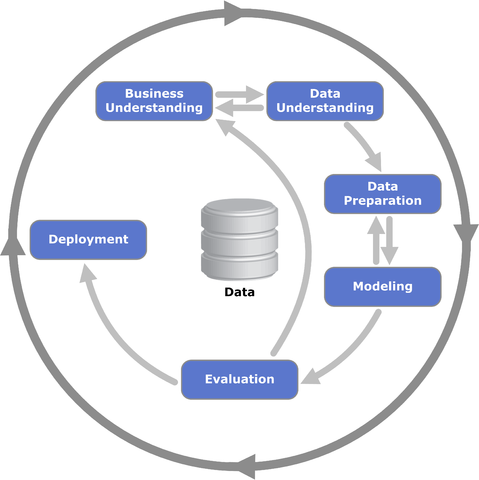
\includegraphics[width=0.5\textwidth,height=\textheight]{Data/CRISP-DM_Process_Diagram1.png}
\caption{CRISP-DM (Source:
\url{https://statistik-dresden.de/archives/1128}))}
\end{figure}

\newpage

\hypertarget{hauptteil}{%
\section{Hauptteil}\label{hauptteil}}

\hypertarget{business-understanding}{%
\subsection{Business Understanding}\label{business-understanding}}

Netzwerkanalyse beschäftigt sich mit der Analyse von verschiedenen Arten
von Netzwerken. Dabei liegt der Fokus auf den Beziehungen und vorallem
den Beziehungsstrukturen zwischen mehreren Knoten. Die Merkmale der
Knoten spielen ebenfalls eine Rolle, das Hauptaugenmerk liegt allerdings
auf den Strukturen und Dynamiken.

\hypertarget{datensatz}{%
\subsubsection{Datensatz}\label{datensatz}}

Der dieser Arbeit zugrunde liegende Datensatz stammt aus der
Datensatz-Bibliothek der Stanford University und bildet ein Netzwerk von
einer Vielzahl an Amazon Produkten. Es handelt sich bei dem Datensatz um
\emph{ready-made Daten}, da der Datensatz als Nebenprodukt einer API
entsteht.\newline ``If a product i is frequently co-purchased with
product j, the graph contains a directed edge from i to j'' \newline Die
Beschreibung des Datensatzes von der Website lässt die Vermutung zu,
dass es Produkte geben muss, welche im Netzwerk zentral sind und häufig
in Verbindung mit anderen Produkten gekauft werden.

\hypertarget{fragestellung}{%
\subsubsection{Fragestellung}\label{fragestellung}}

Aus diesem Grund sollen in dieser Arbeit die folgenden Frage beantwortet
werden:\\

\begin{itemize}
\tightlist
\item
  Welche Produkte werden in Verbindung mit den meisten anderen Produkten
  gekauft?
\item
  Welche Produkte werden hauptsächlich eigenständig gekauft?
\end{itemize}

\hypertarget{data-understanding}{%
\subsection{Data Understanding}\label{data-understanding}}

\hypertarget{laden-der-libraries}{%
\subsubsection{Laden der Libraries}\label{laden-der-libraries}}

Um mit der Datenanalyse und -aufbereitung zu beginnen, müssen zuerst
Libraries geladen, welche relevant sind. \emph{Tidyverse} ist eine
Library, welche eine Vielzahl an Tools in einer eigenen Designphilosophy
mit eigener Grammatik bereitstellt. So gehört zum Beispiel das Paket
\emph{ggplot2} für die Datenvisualisierung zur Libary dazu.
\emph{Tidygraph}, \emph{ggraph} und \emph{igraph} sind für die
Visualisierung notwendig. Das Paket \emph{tinytex} beinhaltet die
Sprache LaTeX für die Kompilierung der Skript-Befehle. Die folgende
Funktion überprüft, ob alle Pakete in der Liste bereits installiert sind
und installiert gegenfalls alle nicht installierten Libraries. Danach
werden alle Libraries geladen.

\begin{Shaded}
\begin{Highlighting}[]
\NormalTok{packages =}\StringTok{ }\KeywordTok{c}\NormalTok{(}\StringTok{"tidyverse"}\NormalTok{, }\StringTok{"tidygraph"}\NormalTok{,}
             \StringTok{"igraph"}\NormalTok{, }\StringTok{"ggraph"}\NormalTok{, }\StringTok{"tinytex"}\NormalTok{)}

\NormalTok{package.check <-}\StringTok{ }\KeywordTok{lapply}\NormalTok{(}
\NormalTok{  packages,}
  \DataTypeTok{FUN =} \ControlFlowTok{function}\NormalTok{(x) \{}
    \ControlFlowTok{if}\NormalTok{ (}\OperatorTok{!}\KeywordTok{require}\NormalTok{(x, }\DataTypeTok{character.only =} \OtherTok{TRUE}\NormalTok{)) \{}
      \KeywordTok{install.packages}\NormalTok{(x, }\DataTypeTok{dependencies =} \OtherTok{TRUE}\NormalTok{)}
      \KeywordTok{library}\NormalTok{(x, }\DataTypeTok{character.only =} \OtherTok{TRUE}\NormalTok{)}
\NormalTok{    \}}
\NormalTok{  \}}
\NormalTok{)}
\end{Highlighting}
\end{Shaded}

\hypertarget{importieren-der-daten}{%
\subsubsection{Importieren der Daten}\label{importieren-der-daten}}

Die Daten stammen aus der Datensatz-Bibliothek der Stanford University
und können als .txt unter folgendem Link heruntergeladen werden. (Link:
\url{https://snap.stanford.edu/data/amazon0302.html})

Zum Einlesen der Daten kommt im Folgenden die Funktion
\textit{read.table} zum Einsatz.\\

\begin{Shaded}
\begin{Highlighting}[]
\NormalTok{amazon <-}\StringTok{ }\KeywordTok{read.table}\NormalTok{(}\StringTok{"Data/Amazon0302.txt"}\NormalTok{)}
\end{Highlighting}
\end{Shaded}

\hypertarget{datenexploration}{%
\subsubsection{Datenexploration}\label{datenexploration}}

Die Daten basieren auf dem Grundsatz ``Kunden, die Artikel A gekauft
haben, haben auch Artikel B gekauft''. Wenn ein Produkt i häufig
zusammen mit Produkt j gekauft wird , enthält der Graph eine gerichtete
Kante von i nach j .

Um einen ersten Einblick in die Daten zu erhalten, wird mit der Funktion
\textit{head} die ersten Zeilen des Datensatzes ausgegeben. Zusätzlich
dazu ist es von entscheidender Rolle, die Qualität der Daten zu
bewerten. Aus diesem Grund werden alle fehlenden Werte, sogenannte NAs
gezählt und ausgegeben.\\

\begin{Shaded}
\begin{Highlighting}[]
\KeywordTok{head}\NormalTok{(amazon)}
\end{Highlighting}
\end{Shaded}

\begin{verbatim}
##   V1 V2
## 1  0  1
## 2  0  2
## 3  0  3
## 4  0  4
## 5  0  5
## 6  1  0
\end{verbatim}

\begin{Shaded}
\begin{Highlighting}[]
\CommentTok{# Count NAs}
\KeywordTok{which}\NormalTok{(}\KeywordTok{is.na}\NormalTok{(amazon))}
\end{Highlighting}
\end{Shaded}

\begin{verbatim}
## integer(0)
\end{verbatim}

Der Dataframe besteht aus 3 Spalten: einer ID Spalte, und zwei
Kantenspalten. Des Weiteren weisen die Daten keine Lücken und fehlenden
Werte auf, sodass der komplette Datensatz für das weitere Vorgehen
genutzt werden kann.

\hypertarget{data-preparation}{%
\subsection{Data Preparation}\label{data-preparation}}

Auf Basis der vorangegangen Schritte müssen nun weitere Anpassungen der
Daten erfolgen, um damit arbeiten zu können. Zum Einen werden die
Kantenspalten von ihren ursprünglichen Namen in sprechendere
Bezeichnungen umbenannt. Im gleichen Schritt werden alle Werte um 1
erhöht, sodass keine Nullen mehr existieren.\\

\begin{Shaded}
\begin{Highlighting}[]
\NormalTok{dat <-}\StringTok{ }\NormalTok{amazon }\OperatorTok\StringTok{ }
\StringTok{  }\KeywordTok{rename}\NormalTok{(}
    \DataTypeTok{from =}\NormalTok{ V1,}
    \DataTypeTok{to =}\NormalTok{ V2}
\NormalTok{  ) }\OperatorTok\StringTok{ }
\StringTok{  }\KeywordTok{mutate}\NormalTok{(}
    \DataTypeTok{from =}\NormalTok{ from}\OperatorTok{+}\DecValTok{1}\NormalTok{,}
    \DataTypeTok{to =}\NormalTok{ to}\OperatorTok{+}\DecValTok{1}
\NormalTok{  )}
\end{Highlighting}
\end{Shaded}

\hypertarget{modeling}{%
\subsection{Modeling}\label{modeling}}

Nach der Datenbearbeitung kann nun das Netz gefittet werden. Hierzu wird
die Funktion \textit{as tbl graph} angewendet, um ein Netz zu
erstellen.\\

\begin{Shaded}
\begin{Highlighting}[]
\NormalTok{net <-}\StringTok{ }\KeywordTok{as_tbl_graph}\NormalTok{(dat)}
\NormalTok{net}
\end{Highlighting}
\end{Shaded}

\begin{verbatim}
## # A tbl_graph: 262111 nodes and 1234877 edges
## #
## # A directed simple graph with 1 component
## #
## # Node Data: 262,111 x 1 (active)
##   name 
##   <chr>
## 1 1    
## 2 2    
## 3 3    
## 4 4    
## 5 5    
## 6 6    
## # ... with 262,105 more rows
## #
## # Edge Data: 1,234,877 x 2
##    from    to
##   <int> <int>
## 1     1     2
## 2     1     3
## 3     1     4
## # ... with 1,234,874 more rows
\end{verbatim}

Die beiden Spalten aus dem Ursprungsdatensatz wurden in ein Netz,
bestehend aus 262111 Knoten und 1234877 Kanten, konvertiert. Es handelt
sich, wie aus der Zusammenfassung des Netzes zu entnehmen ist, um einen
gericheteten Graphen. Die Knotennamen sind in diesem Fall die Ziffern
der Kantendaten. Leider liegt dem Autor dieser Arbeit keine
Zuordnungsliste von Knotenziffern zu realen Amazonprodukten vor. Aus
diesem Grund wird im Folgenden mit den Ziffern der Knoten
weitergearbeitet.\\

\begin{Shaded}
\begin{Highlighting}[]
\CommentTok{# Calculate Degree of Vertices}
\NormalTok{degree <-}\StringTok{ }\KeywordTok{degree}\NormalTok{(net)}

\CommentTok{# Adjacency Matrix}
\NormalTok{adjacencyMatrix <-}\StringTok{ }\NormalTok{net[]}
\end{Highlighting}
\end{Shaded}

Aus dem Netz kann nun der Degree abgeleitet und abgespeichert werden.
Der Degree oder Grad eines Knoten ist die Anzahl von Kanten, die an ihn
angrenzen. Für die Analyse ist die Verteilung der Grade der Knoten
interessant. Gibt es eine überwiegende Mehrheit an Knoten, welche die
gleiche Anzahl an Kanten besitzen? Gibt es Ausreißer mit vielen Kanten?
Ähnelt die Verteilung einer Normalverteilung, ist die links oder rechts
verschoben?\\
Um diese Fragen zu beantworten, wird im nächsten Schritt ein Histogramm
erzeugt, welches die Knotengrade des Netzwerkes visualisiert.\\

\hypertarget{data-visualization}{%
\subsection{Data Visualization}\label{data-visualization}}

Um die Degrees für die Visualisierung nutzen zu können, müssen diese
zuvor in ein Dataframe umgewandelt werden. Dies geschieht mit der
Funktion \emph{as.data.frame}. Anschließend wird die Library
\emph{ggplot2} für das Histogramm angewendet.

\begin{Shaded}
\begin{Highlighting}[]
\NormalTok{degree_df <-}\StringTok{ }\KeywordTok{as.data.frame}\NormalTok{(degree)}


\NormalTok{hist_of_degrees <-}\StringTok{ }\KeywordTok{ggplot}\NormalTok{(}\DataTypeTok{data =}\NormalTok{ degree_df, }\KeywordTok{aes}\NormalTok{(}\DataTypeTok{x=}\NormalTok{degree))}\OperatorTok{+}
\StringTok{  }\KeywordTok{geom_bar}\NormalTok{(}\DataTypeTok{fill =} \StringTok{"#e2001a"}\NormalTok{, }\DataTypeTok{colour =} \StringTok{"#e2001a"}\NormalTok{, }\DataTypeTok{alpha=}\NormalTok{.}\DecValTok{5}\NormalTok{)}\OperatorTok{+}
\StringTok{  }\KeywordTok{scale_y_continuous}\NormalTok{(}\DataTypeTok{trans=}\StringTok{'log10'}\NormalTok{)}\OperatorTok{+}
\StringTok{  }\KeywordTok{xlim}\NormalTok{(}\DecValTok{0}\NormalTok{,}\DecValTok{120}\NormalTok{)}\OperatorTok{+}
\StringTok{  }\KeywordTok{labs}\NormalTok{(}\DataTypeTok{title =} \StringTok{"Histogram of Node-Degrees"}\NormalTok{, }
       \DataTypeTok{subtitle =} \StringTok{"Amazon Network Analysis"}\NormalTok{, }
       \DataTypeTok{y =} \StringTok{"Frequency (log10 scale)"}\NormalTok{, }
       \DataTypeTok{x =} \StringTok{"Degree of Vertices (xlim = 120)"}\NormalTok{)}\OperatorTok{+}
\StringTok{  }\KeywordTok{theme_classic}\NormalTok{()}

\NormalTok{hist_of_degrees}
\end{Highlighting}
\end{Shaded}

\begin{figure}
\centering
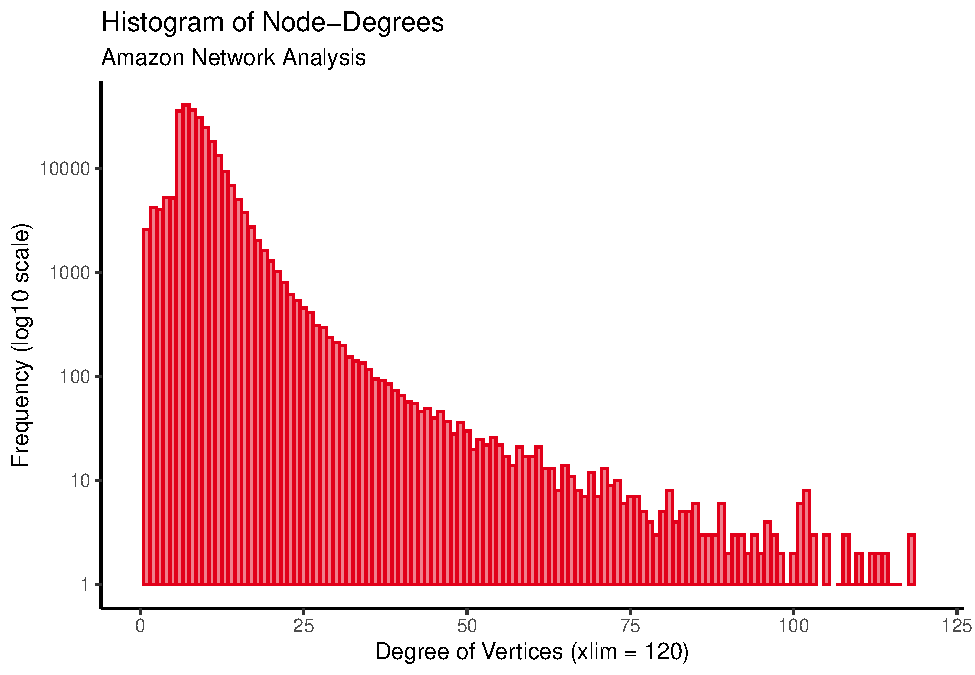
\includegraphics{Assignment_files/figure-latex/viz-1.pdf}
\caption{Knotengrad Histogramm}
\end{figure}

Das Histogramm der Knotengrade zeigt eine Mehrheit der Grade im Bereich
5-20. Dies bedeutet, dass eine Mehrheit der Knoten im Datensatz eine
durchschnittliche Anzahl an Kanten von 5-20 aufweist. Weiterhin ist zu
erkennen, dass einige Knoten 100 und mehr Kanten besitzen. Die großen
Ausreißer wurden in diesem Plot weggelassen, doch selbst in dieser
Darstellungsweise zeigt sich ein abflachender Bereich Richtung x
--\textgreater{} unendlich. Um eine übersichtlichere Darstellung der
Observationen um den Nullbereich der y-Achse zu gewährleisten, wurde die
y-Achse nach dem dekadischen Logarithmus skaliert.

\hypertarget{experimental-data}{%
\subsection{Experimental Data}\label{experimental-data}}

Um die Laufzeit und die Übersichtlichkeit der Visualisierungen zu
verbessern hat sich der Autor dieser Arbeit dazu entschieden, die
Fragestellung anhand einer Teilmenge des gesamten Datensatzes
durchzuführen. Es wird demnach ein Subset von \emph{250 Zeilen} aus dem
Datensatz verwendet.

\begin{Shaded}
\begin{Highlighting}[]
\CommentTok{# Subsetting Data}
\NormalTok{dat_exp <-}\StringTok{ }\NormalTok{dat[}\DecValTok{1}\OperatorTok{:}\DecValTok{250}\NormalTok{,]}

\NormalTok{net_exp <-}\StringTok{ }\KeywordTok{as_tbl_graph}\NormalTok{(dat_exp)}

\NormalTok{net_exp <-}\StringTok{ }\NormalTok{net_exp }\OperatorTok\StringTok{ }
\StringTok{  }\KeywordTok{activate}\NormalTok{(nodes) }\OperatorTok\StringTok{ }
\StringTok{  }\KeywordTok{mutate}\NormalTok{(}
    \DataTypeTok{degree =} \KeywordTok{centrality_degree}\NormalTok{()}
\NormalTok{  )}
\end{Highlighting}
\end{Shaded}

\hypertarget{zentralituxe4tsmauxdf}{%
\subsubsection{Zentralitätsmaß}\label{zentralituxe4tsmauxdf}}

Um die Fragestellung dieser Arbeit zu beantworten, müssen weitere
Erkenntnisse über die Netzwerk-Struktur analysiert werden. Hierfür sind
Zentralitätsmaße eine gute Anlaufstelle, um ``wichtigere Knoten'' im
Sinne des Maßes zu identifizieren. Der Autor hat sich für die
Beantwortung der Fragestellung:\\
\emph{Welche Produkte werden in Verbindung mit den meisten anderen
Produkten gekauft?}\\
für die Betweenness-Centrality entschieden. Ein Knoten hat einen hohen
Betweenness-Wert, wenn dieser Knoten Bestandteil besonders vieler
kürzester Wege ist und die jeweiligen Paare wenige andere kürzeste Wege
haben, auf der der Knoten nicht enthalten ist. Für jedes Paar von Knoten
wird daher der Anteil an kürzesten Wegen zwischen ihnen berechnet, die v
enthalten. Diese Anteile werden für alle Paare von Knoten aufsummiert um
die Betweennesszentralität von v zu berechnen.

\begin{Shaded}
\begin{Highlighting}[]
\CommentTok{# Betweenness Centrality}
\NormalTok{centr_betweenness <-}\StringTok{ }\KeywordTok{betweenness}\NormalTok{(}
\NormalTok{  net_exp,}
  \DataTypeTok{directed =} \OtherTok{TRUE}\NormalTok{,}
  \DataTypeTok{weights =} \OtherTok{NULL}\NormalTok{,}
  \DataTypeTok{nobigint =} \OtherTok{TRUE}\NormalTok{,}
  \DataTypeTok{normalized =} \OtherTok{FALSE}
\NormalTok{)}

\NormalTok{df_centr_betweenness <-}\StringTok{ }\KeywordTok{as.data.frame}\NormalTok{(centr_betweenness)}

\NormalTok{top_}\DecValTok{5}\NormalTok{ <-}\StringTok{ }\NormalTok{df_centr_betweenness }\OperatorTok\StringTok{ }
\StringTok{  }\KeywordTok{top_n}\NormalTok{(}\DecValTok{5}\NormalTok{)  }\CommentTok{# highest values}

\NormalTok{top_}\DecValTok{5}
\end{Highlighting}
\end{Shaded}

\begin{verbatim}
##    centr_betweenness
## 9          1154.5000
## 12          343.0667
## 21          585.7333
## 23          470.0000
## 31          428.7500
\end{verbatim}

Zu sehen sind die fünf Knoten der Teilmenge des Datensatzes mit den
höchsten Betweenness-Zentralitätsmaßen. Dies bedeutet, dass Knoten
Nummer 9 der Knoten ist, welcher die größte Bedeutung im Bezug auf die
meisten kürzesten Wege hat. In dieser Teilmenge des Datensatzes ist
Knoten Nummer 9 das Produkt, welches am meisten in Verbindung mit
anderen Produkten gekauft wird.

\hypertarget{visualisierung}{%
\subsubsection{Visualisierung}\label{visualisierung}}

Um die Beziehungen des Knoten Nummer 9 besser verstehen zu können,
werden im Folgenden drei Visualisierungen erstellt.\\

\begin{Shaded}
\begin{Highlighting}[]
\CommentTok{# Data Viz for Subset}
\CommentTok{# network diagramm}
\KeywordTok{ggraph}\NormalTok{(net_exp, }\DataTypeTok{layout =} \StringTok{'fr'}\NormalTok{, }\DataTypeTok{maxiter =} \DecValTok{100}\NormalTok{) }\OperatorTok{+}\StringTok{ }
\StringTok{  }\KeywordTok{geom_node_point}\NormalTok{(}\DataTypeTok{colour=}\StringTok{"#e2001a"}\NormalTok{) }\OperatorTok{+}\StringTok{ }
\StringTok{  }\KeywordTok{geom_edge_link}\NormalTok{(}\DataTypeTok{alpha =} \FloatTok{.4}\NormalTok{) }\OperatorTok{+}
\StringTok{  }\KeywordTok{geom_node_label}\NormalTok{(}\KeywordTok{aes}\NormalTok{(}\DataTypeTok{label=}\KeywordTok{ifelse}\NormalTok{(name }\OperatorTok{==}\StringTok{ "9"}\NormalTok{, name, }\OtherTok{NA}\NormalTok{))) }\OperatorTok{+}
\StringTok{  }\KeywordTok{theme_graph}\NormalTok{()}
\end{Highlighting}
\end{Shaded}

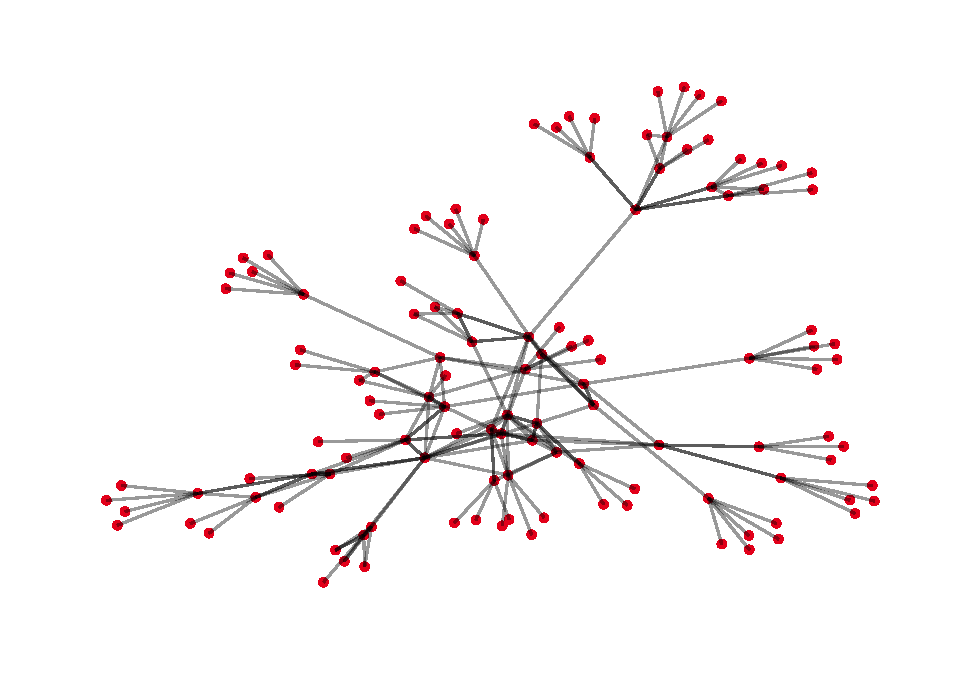
\includegraphics{Assignment_files/figure-latex/unnamed-chunk-2-1.pdf}
\newpage

\begin{Shaded}
\begin{Highlighting}[]
\KeywordTok{ggraph}\NormalTok{(net_exp, }\DataTypeTok{layout =} \StringTok{'kk'}\NormalTok{, }\DataTypeTok{maxiter =} \DecValTok{100}\NormalTok{) }\OperatorTok{+}\StringTok{ }
\StringTok{  }\KeywordTok{geom_node_point}\NormalTok{(}\DataTypeTok{colour=}\StringTok{"#e2001a"}\NormalTok{) }\OperatorTok{+}\StringTok{ }
\StringTok{  }\KeywordTok{geom_edge_link}\NormalTok{(}\DataTypeTok{alpha =} \FloatTok{.4}\NormalTok{) }\OperatorTok{+}
\StringTok{  }\KeywordTok{geom_node_label}\NormalTok{(}\KeywordTok{aes}\NormalTok{(}\DataTypeTok{label=}\KeywordTok{ifelse}\NormalTok{(name }\OperatorTok{==}\StringTok{ "9"}\NormalTok{, name, }\OtherTok{NA}\NormalTok{))) }\OperatorTok{+}
\StringTok{  }\KeywordTok{theme_graph}\NormalTok{()}
\end{Highlighting}
\end{Shaded}

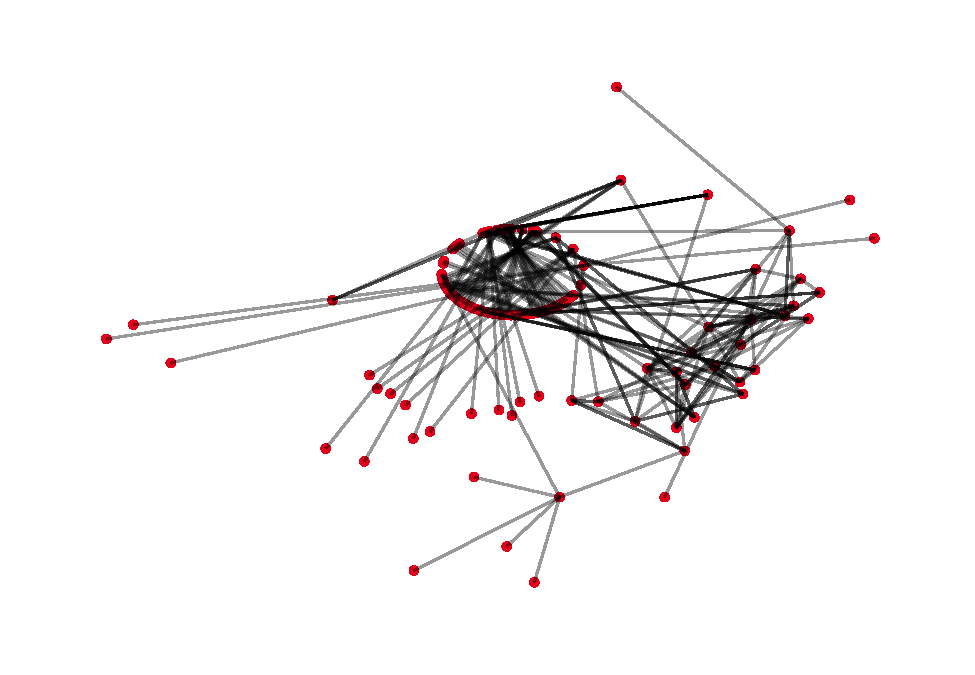
\includegraphics{Assignment_files/figure-latex/unnamed-chunk-3-1.pdf}
\newpage

\begin{Shaded}
\begin{Highlighting}[]
\CommentTok{# coord diagramm}
\KeywordTok{ggraph}\NormalTok{(net_exp, }\DataTypeTok{layout =} \StringTok{'linear'}\NormalTok{, }\DataTypeTok{circular =} \OtherTok{TRUE}\NormalTok{) }\OperatorTok{+}\StringTok{ }
\StringTok{  }\KeywordTok{geom_node_point}\NormalTok{(}\DataTypeTok{colour=}\StringTok{"#e2001a"}\NormalTok{) }\OperatorTok{+}
\StringTok{  }\KeywordTok{geom_edge_arc}\NormalTok{(}\DataTypeTok{alpha =} \FloatTok{.4}\NormalTok{) }\OperatorTok{+}
\StringTok{  }\KeywordTok{geom_node_label}\NormalTok{(}\KeywordTok{aes}\NormalTok{(}\DataTypeTok{label=}\KeywordTok{ifelse}\NormalTok{(name }\OperatorTok{==}\StringTok{ "9"}\NormalTok{, name, }\OtherTok{NA}\NormalTok{))) }\OperatorTok{+}
\StringTok{  }\KeywordTok{theme_graph}\NormalTok{()}
\end{Highlighting}
\end{Shaded}

\begin{figure}
\centering
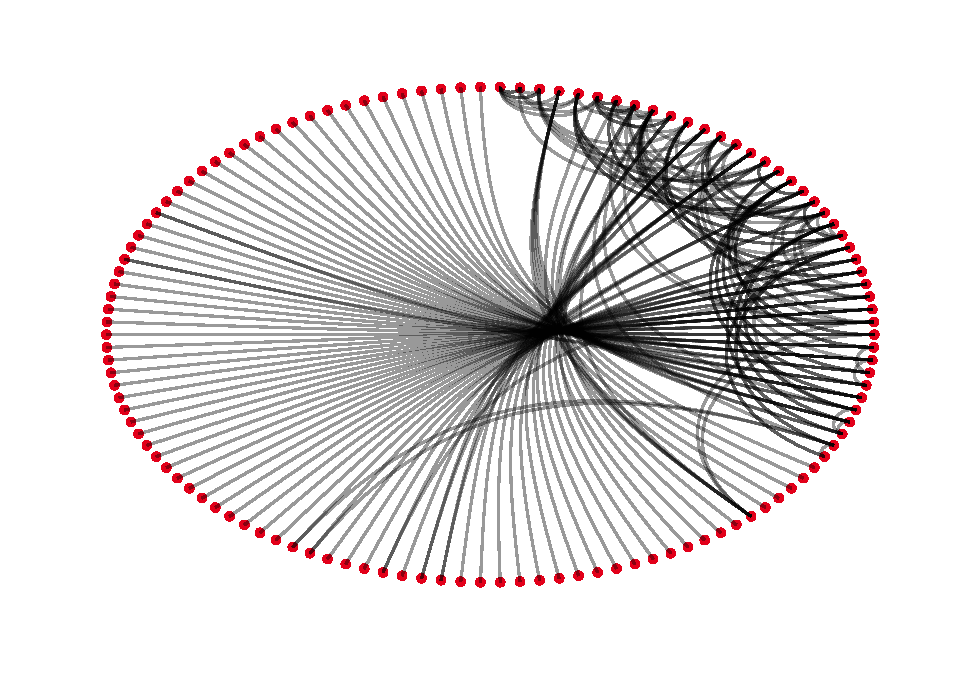
\includegraphics{Assignment_files/figure-latex/unnamed-chunk-4-1.pdf}
\caption{Netzwerk Visualisierung 3}
\end{figure}

\newpage

\hypertarget{fazit}{%
\section{Fazit}\label{fazit}}

\hypertarget{evaluation-der-ergebnisse}{%
\subsection{Evaluation der Ergebnisse}\label{evaluation-der-ergebnisse}}

tbd

\hypertarget{kritische-reflexion}{%
\subsection{kritische Reflexion}\label{kritische-reflexion}}

tbd

\end{document}
